\textbf{Цель работы:} с помощью сцинтиляционного спектрометра исследуется энергетический спектр $\gamma$-квантов, рассеянных на графите. Опреляется энергия рассеянных $\gamma$-квантов в зависимости от угла рассеяния, а также энергия покоя частиц, на которых происходит комптоновское рассеяние.

\section{Теоретическое введение}

    Эффект Комптона -- увеличение длины волны рассеянного излучения по сравнению с падающим -- интерпретируется как результат упругого содуранеия двух частиц: $\gamma$-кванта и свободного электрона.
	
	Из закона сохранения 4-имульса для системы <<фотон + электрон>> следует формула для изменения длины волны рассеянного излучения:
	\begin{equation}
		\label{Kompton}
		\tag{$\star$}
		\Delta \lambda = \Lambda_K(1-\cos\theta),
	\end{equation}
	где величина $\Lambda_K = h/(mc) = 2,42 \cdot 10^{-10}$ см называется комптоновской длиной волны электрона.
	
	Из формулы \eqref{Kompton} следует, что комптоновское смещение не зависит ни от длины волны первичного излучения, ни от рода вещества, в котором наблюдается рассеяние. В общем случае комптоновоское рассеяние происходит на свободных электронах в атоме. Для $\gamma$-квантов с энергией в несколько десятков, а тем более сотен килоэлектрон-вольт, связь электронов в атоме мало существенна, так как энергрия их связи в легких атомах не превосходит нескольких килоэлектрон-вольт, а для большинства электронов еще меньше.
	
	При рассеянии на связанных электронах изменение импульса кванта воспринимается атомом в целом. Посколько масса атома очень велика, переда ча импульса не спровождается сколь-нибудь заметной передачей энергии, и наблюдается несмещенная (по энергии) компонента в спектре рассеянного излучения. Таким образом, рассеяние $\gamma$-квантов на связанных электронах можно рассматривать как упругое столкновение квантов с атомами.
	
	Основной целью данной работы является проверка соотношения \eqref{Kompton}. Применительно к условиям нашего опыта формулу \eqref{Kompton} следует преобразовать от длин волн к энергиям $\gamma$-квантов. Как нетрудно показать, соответсвующиее выражение имеет вид:
	\begin{equation}
		\label{1-cos}
		\tag{$\star\star$}
		\frac{1}{\varepsilon(\theta)} - \frac{1}{\varepsilon_0} = 1 - \cos \theta.
	\end{equation}

	Здесь $\varepsilon_0 = E_0/(mc^2)$ -- выраженная в единицах $(mc^2)$ энергия $\gamma$-квантов, падающих на рассеиватель, $\varepsilon(\theta)$ -- выраженная в тех же единицах энергия квантов, испытавших комптоновское рассеяние на угол $\theta$, $m$ -- масса электрона.
	
	Заменим в формуле \eqref{1-cos} энергию квантов, испытавших комптоновское рассеяние на угол $\theta$, номером канала $N(\theta)$, соответствующего вершине фотопика при указанном угле $\theta$:
	\begin{equation}
		\label{kek}
		\tag{$\star \star \star$}
		\frac{1}{N(\theta)} - \frac{1}{N(0)} = A (1 - \cos \theta),
	\end{equation}
	где $A$ -- неизвестный коэффциицент пропорциональности между $\varepsilon(\theta)$ и $N(\theta)$.

\section{Экспериментальная установка}

    Блок-схема установки изображена на рис.~\ref{exp_scheme}. Источником излучения 1 служит $^{137}$Cs, испускающий $\gamma$-лучи с энергией 662 кэВ. Он помещен в толстенный свинцовый контейнер с коллиматором. Сформмированный коллиматором узкий пучок $\gamma$-квантов попадает на графитовую мишень 2 (цилиндр диамтером 40 мм и высотой 100 мм.)

    \begin{figure}[h!]
        \centering
        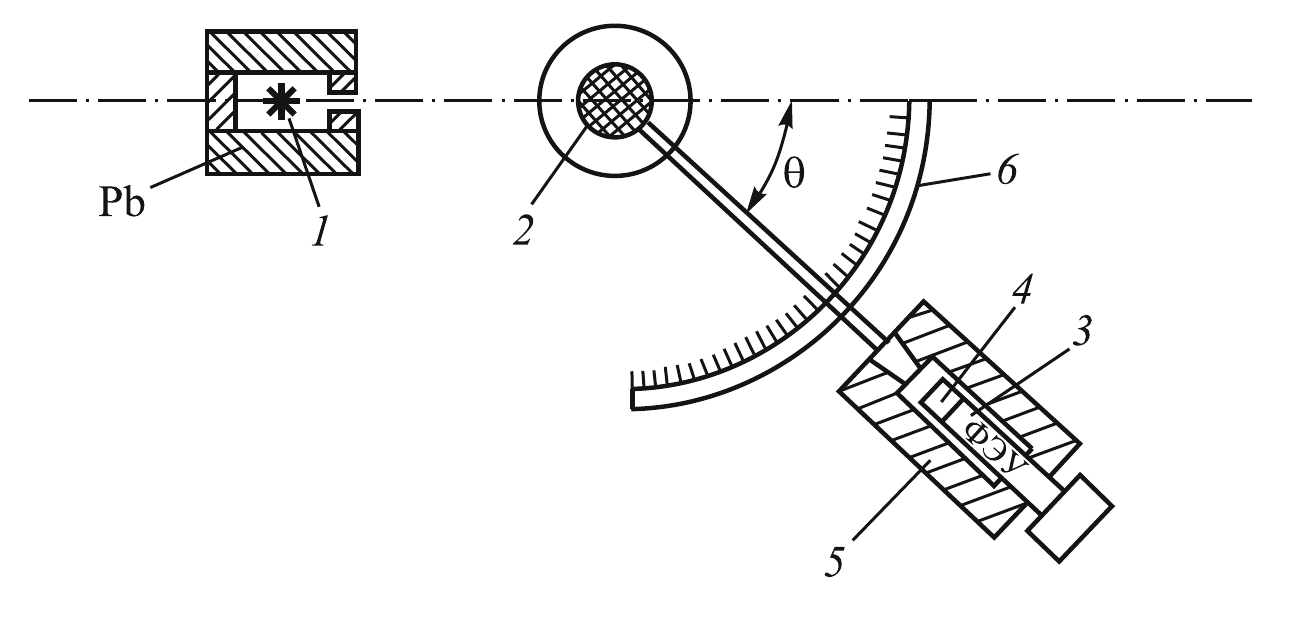
\includegraphics[width = 12 cm]{images/exp_scheme}
        \caption{Блок-схема экспериментальной установки}
        \label{exp_scheme}
    \end{figure}

    \begin{figure}[h!]
        \centering
        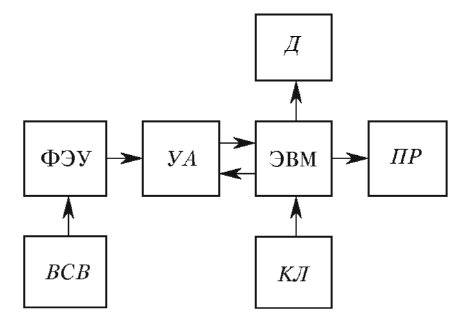
\includegraphics[width = 8 cm]{images/exp_measure_scheme}
        \caption{Блок-схема измерительного комплекса}
        \label{exp_measure_scheme}
    \end{figure}
    
	Кванты, испытавшие комптоновское рассеяние в мишени, региструруются сцинтилляционным счетчиком. Счетчик состоит из фотоэлектронного умножителя 3 (далее ФЭУ) и сцинтиллятора 4. Сцинтиллятором служит кристалл NaI(Tl) цилиндрической формы диаметром 40 мм и высотой 40 мм, его выходное окно находится в оптическом контакте с фотокатодом ФЭУ. Сигналы, возникающие на ФЭУ, подаются на ЭВМ для амплитудного анализа. Кристалл и ФЭУ расположены в светонепроницаемом блоке, укрепленном на горизонтальной штанге. Штанга вместе с этим блоком может вращаться относительно мишени, угол поворота отсчитывается по лимбу 6.
	
	На рис.~\ref{exp_measure_scheme} представлена функциональная блок-схема измерительного комплекса, который состоит из ФЭУ, питаемого от высоковольтного выпрямителя ВСВ, обеспечивающего работу ФЭУ в спектрометрическом режиме, усилителя-анализатора УА, являющегося входным интерфейсом ЭВМ, управляемой с клавиатуры КЛ. В ходе проведения эксперимента информация отражается на экране дисплея Д, окончательные результаты в виде таблиц и графиков могут быть выведены на принтер ПР.
	
\section{Ход работы}

	С помощью установки снимем зависимость $N(\theta)$, которая имеет следующий вид:

	\begin{figure}[H]
		\centering
		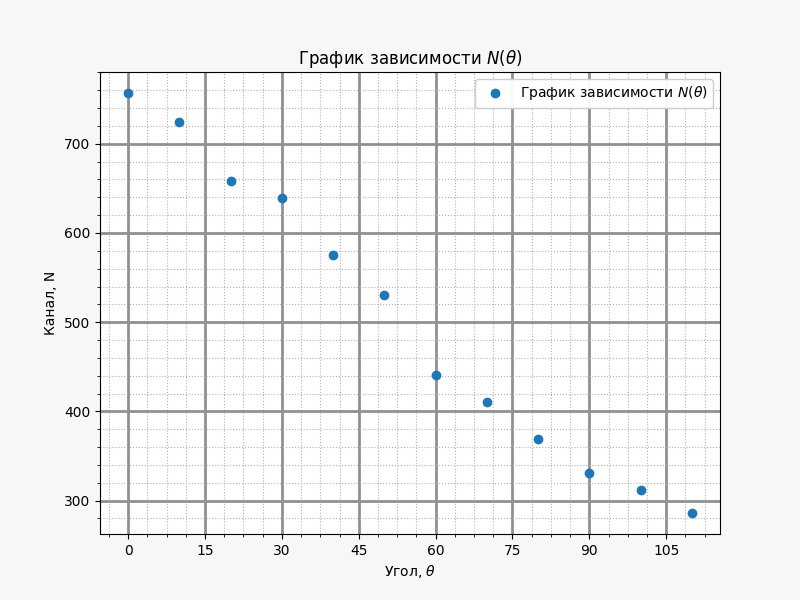
\includegraphics[width = 11.5 cm]{images/N_theta}
		\caption{График зависимости $N(\theta)$}
		\label{N_theta}
	\end{figure}

	Теперь проверим выполнимость формулы Комптона:

	\begin{figure}[H]
		\centering
		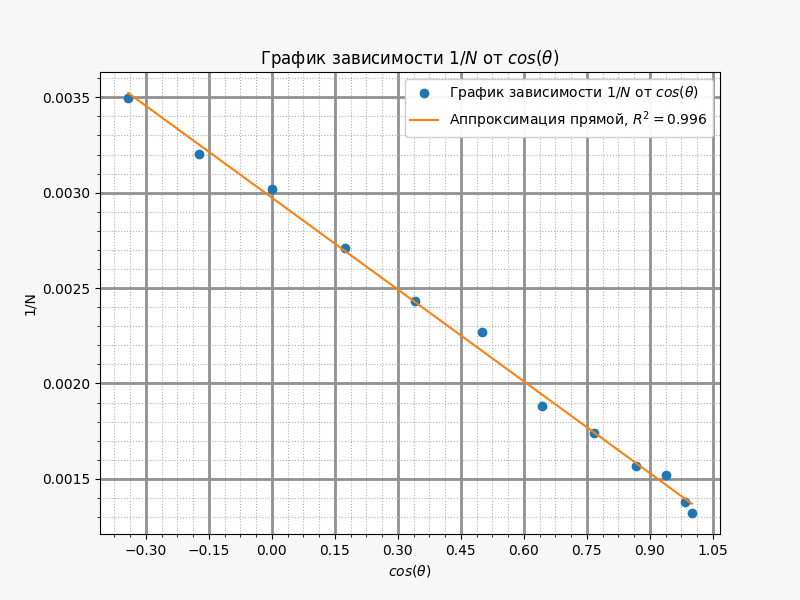
\includegraphics[width = 12 cm]{images/N_inv_theta}
		\caption{График зависимости $1/N$ от $cos(\theta)$}
		\label{N_inv_theta}
	\end{figure}

	Таким образом, выполняется линейная комптоновская зависимость $1/N \thicksim 1/\varepsilon$ от $cos(\theta)$ с коэффициентом корелляции $R^2 = 0.996$:
	\begin{equation}
		\frac{1}{N} = b - a \cdot \cos \theta, \; b = (2.97 \pm 0.10) \cdot 10^{-3}, a = (1.60 \pm 0.06) \cdot 10^{-3}
	\end{equation}

	Теперь определим энергию покоя частицы, на которой происходит комптоновское рассеяние, воспользовавшись формулой Комптона:
	\begin{equation}
		mc^2 = \varepsilon(0) \frac{\varepsilon(90)}{\varepsilon(0) - \varepsilon(90)} = \varepsilon(0) \frac{N(90)}{N(0) - N(90)}, \; \varepsilon(0) = \varepsilon_{Cs} = 662 \; \text{КэВ}
	\end{equation}
	\begin{equation*}
		N(0) = \frac{1}{b - a} = (0.730 \pm 0.084) \cdot 10^3, \; N(90) = \frac{1}{b} = (0.337 \pm 0.011) \cdot 10^3
	\end{equation*}
	\begin{equation}
		mc^2 = (567 \pm 155) \; \text{КэВ}
	\end{equation}

	Полученное значение в пределах погрешности совпадает с табличным значением энергии покоя электрона $mc^2 = 511$ КэВ.

\section{Заключение}

	Таким образом, проверена комптоновкая зависимость энергии рассеянного фотона от угла рассения, а также найдено значение энергии покоя электрона
	\begin{equation}
		mc^2 = (567 \pm 155) \; \text{КэВ},
	\end{equation}
	которое в пределах погрешности совпадает с табличным значением энергии покоя электрона $mc^2 = 511$ КэВ.